\documentclass{beamer}
\usetheme{Boadilla}
\usepackage[utf8x]{inputenc}
\usepackage{listings}
\title{LS IoT Platform}
\subtitle{Piattaforma per il monitoraggio di macchine utensili con integrazione a software ERP Microsoft Dynamics NAV}
\author{Vincenzo Nucci e Matteo Tiberi}
%\author{Matteo Tiberi}
\institute{Università di Camerino}

\begin{document}
	\begin{frame}
		\titlepage
	\end{frame}

\begin{frame}
\frametitle{LS IoT Platform}
	\begin{itemize}
		\item espone servizi REST per letture di sensori
		\begin{itemize}
			\item ultima lettura di un sensore
			\item letture di una certa settimana
			\item letture di un certo mese
			\item letture di determinati campi dei sensori
		\end{itemize}
		\item servizio di sottoscrizione con notifiche PUSH
		\begin{itemize}
			\item debolmente accoppiato grazie ad Apache ActiveMQ
		\end{itemize}
		\item integrazione della sottoscrizione con Microsoft Dynamics NAV
		\begin{itemize}
			\item utilizzo dei web services SOAP offerti da NAV
		\end{itemize}
		\item indipendente da sorgenti dati e formato dei dati
		\begin{itemize}
			\item grazie alle interfacce e Apache Avro
		\end{itemize}
		\item interfaccia web
		\begin{itemize}
			\item pagina per la registrazione delle applicaizoni
			\item pagina per la gestione delle richieste
			\item pagina per la gestione dei servizi attivi per gli utenti
		\end{itemize}
	\end{itemize}
\end{frame}

\begin{frame}
\frametitle{Pagina web di richiesta token}
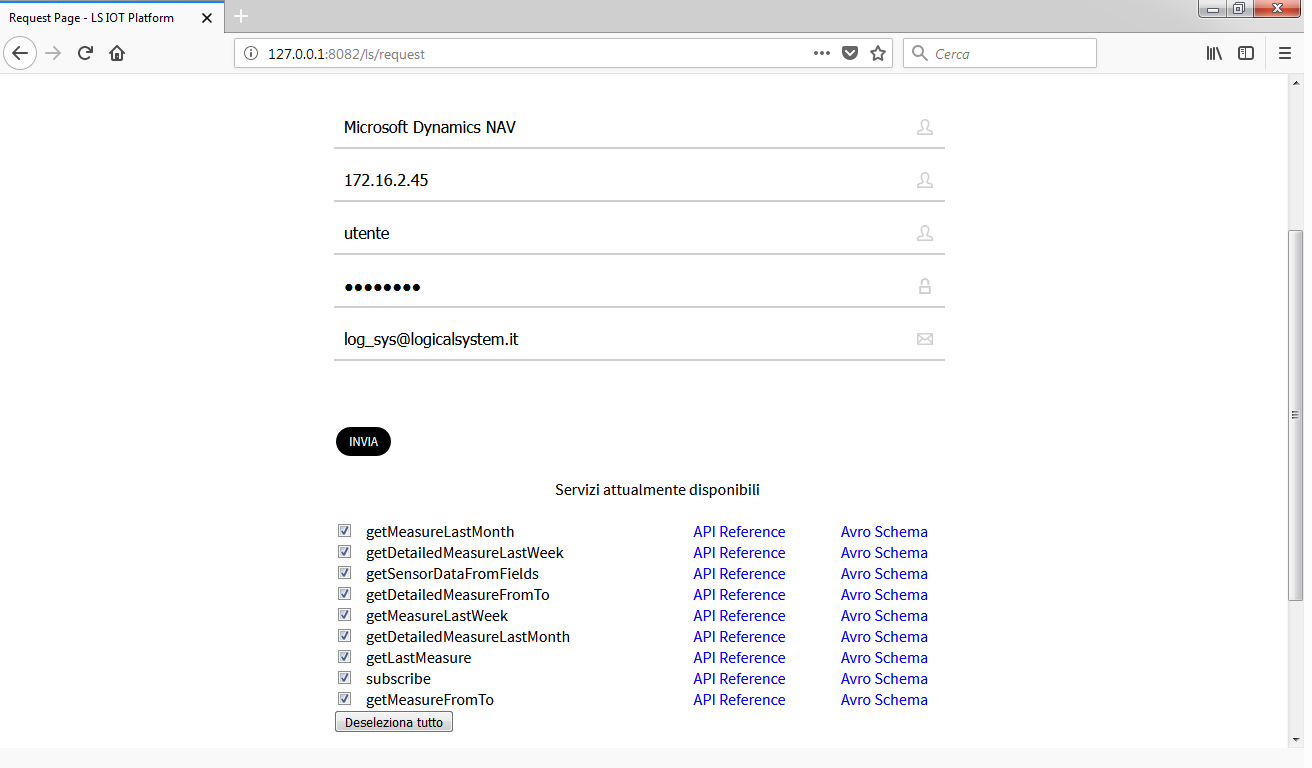
\includegraphics[width=1\textwidth]{images/RequestPagePlatform.png}
\end{frame}

\begin{frame}
\frametitle{Richieste database}
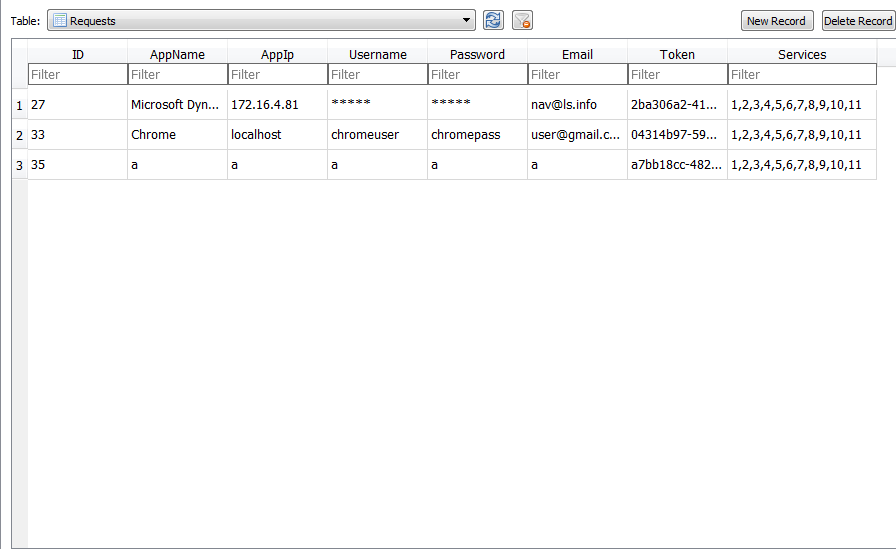
\includegraphics[width=1\textwidth]{images/DBPlatform2.png}
\end{frame}

\begin{frame}
\frametitle{Pagina web gestione delle richieste}
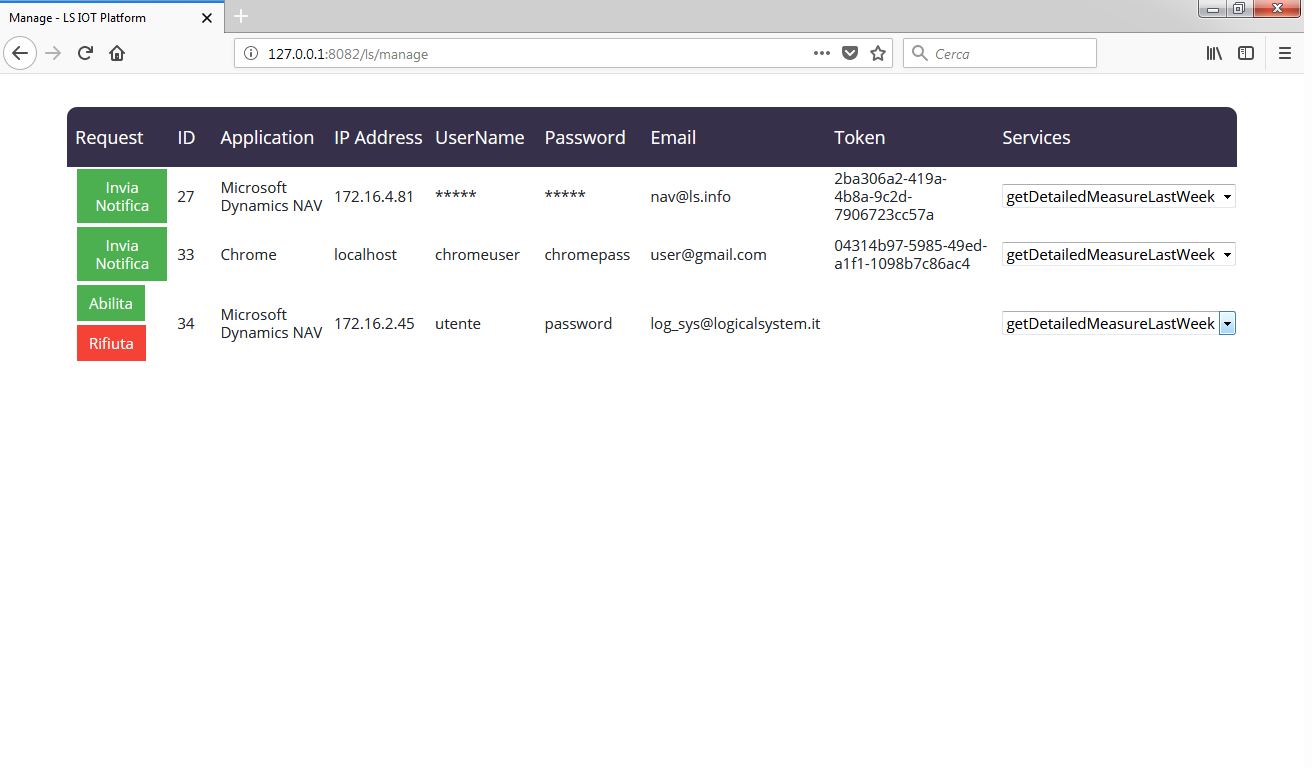
\includegraphics[width=1\textwidth]{images/managePagePlatform.png}
\end{frame}

\begin{frame}
\frametitle{Sottoscrizioni database}
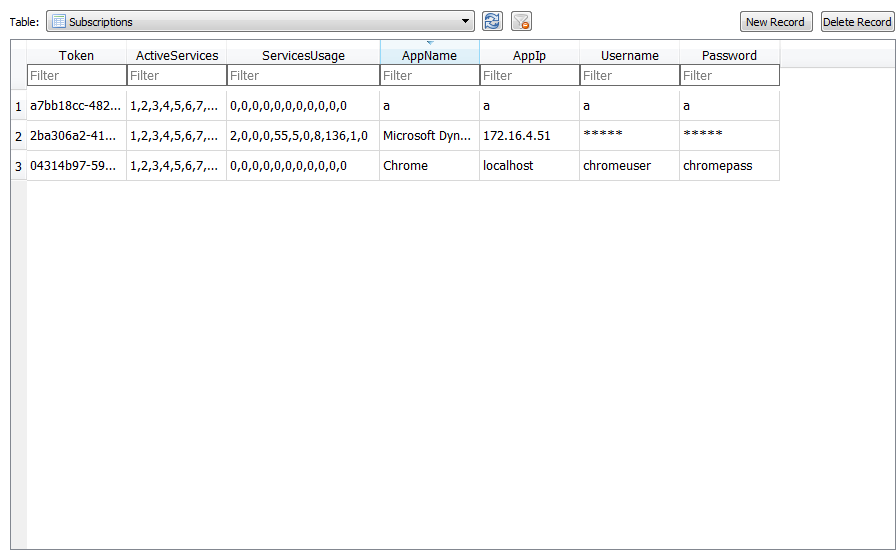
\includegraphics[width=1\textwidth]{images/DBPlatform3.png}
\end{frame}

\begin{frame}
\frametitle{Pagina web gestione dei servizi utenti}
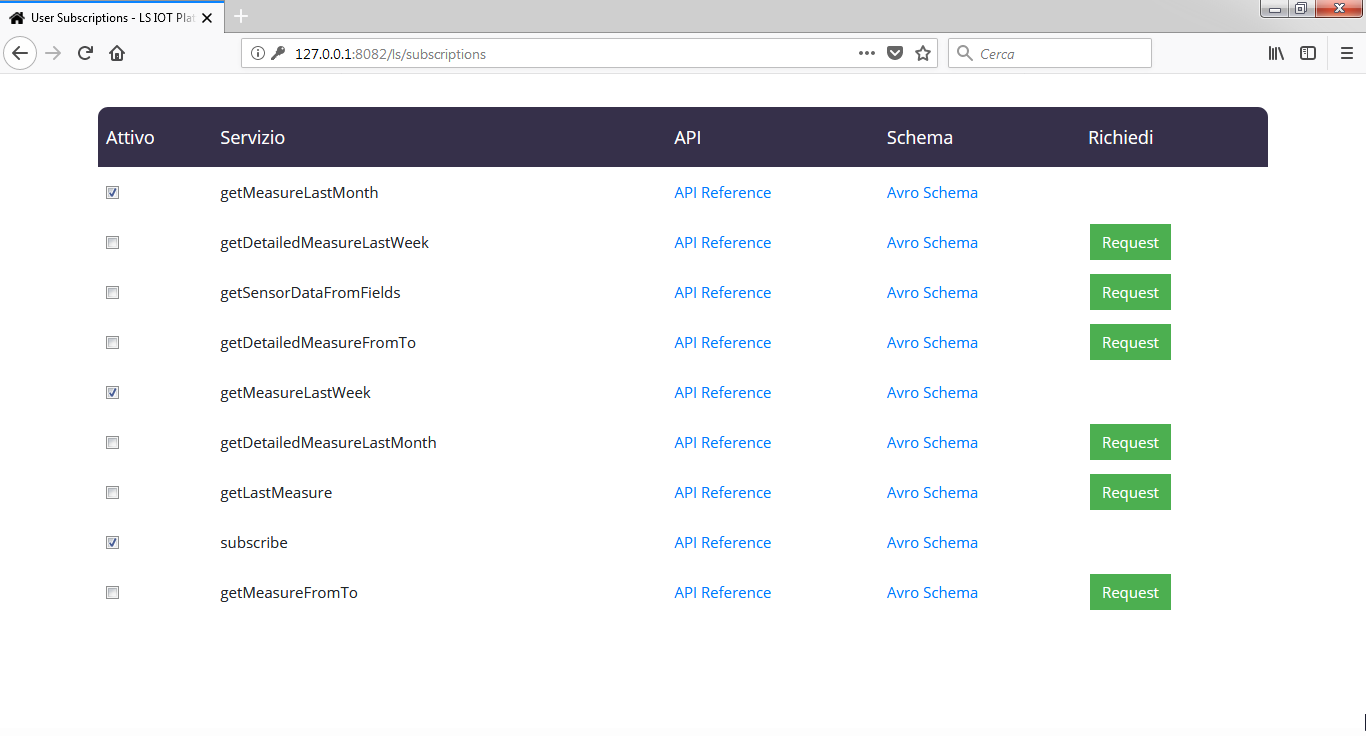
\includegraphics[width=1\textwidth]{images/UserSubscriptionsPlatform.png}
\end{frame}

\begin{frame}
\frametitle{Esempio di un servizio}
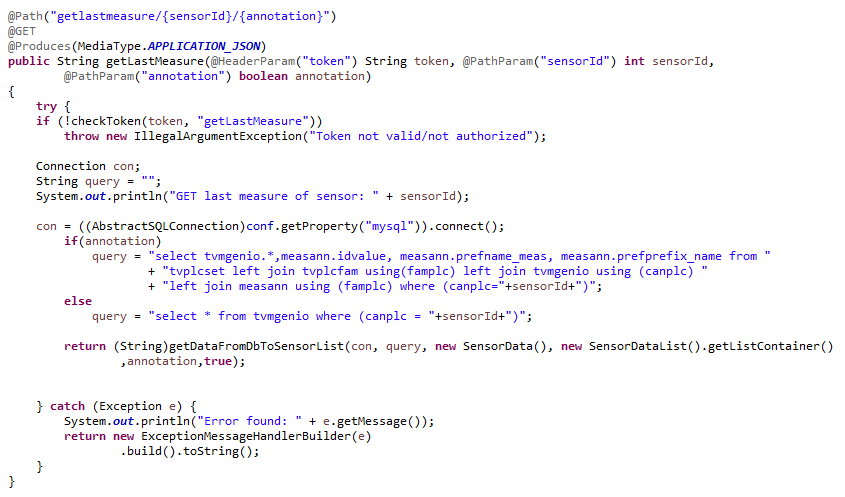
\includegraphics[width=1\textwidth]{images/getlastmeasure.png}
\end{frame}

\begin{frame}
\frametitle{Risposta chiamata getlastmeasure}
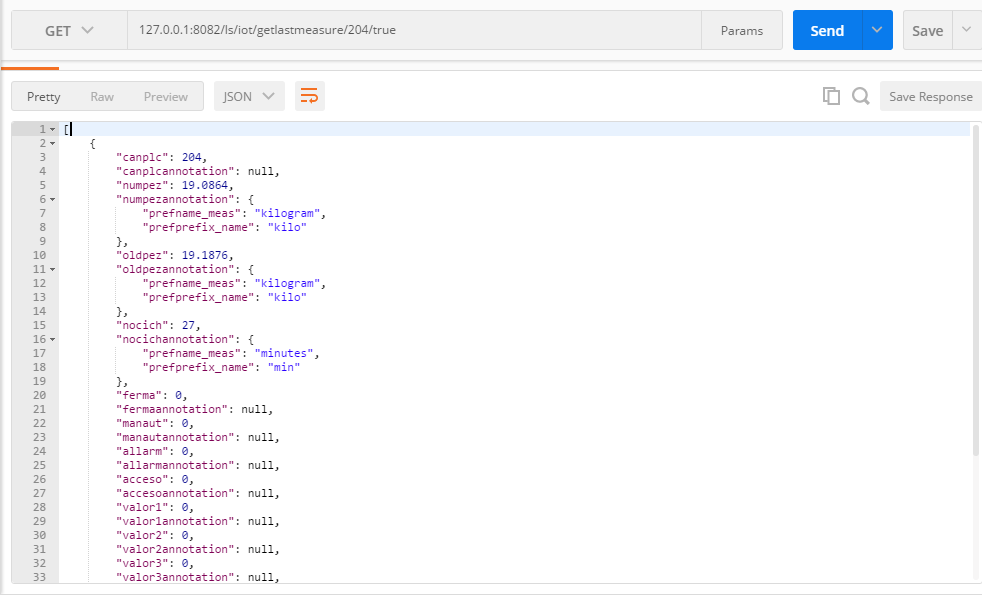
\includegraphics[width=1\textwidth]{images/Postman1.png}
\end{frame}

\begin{frame}
\frametitle{Smart Object Page}
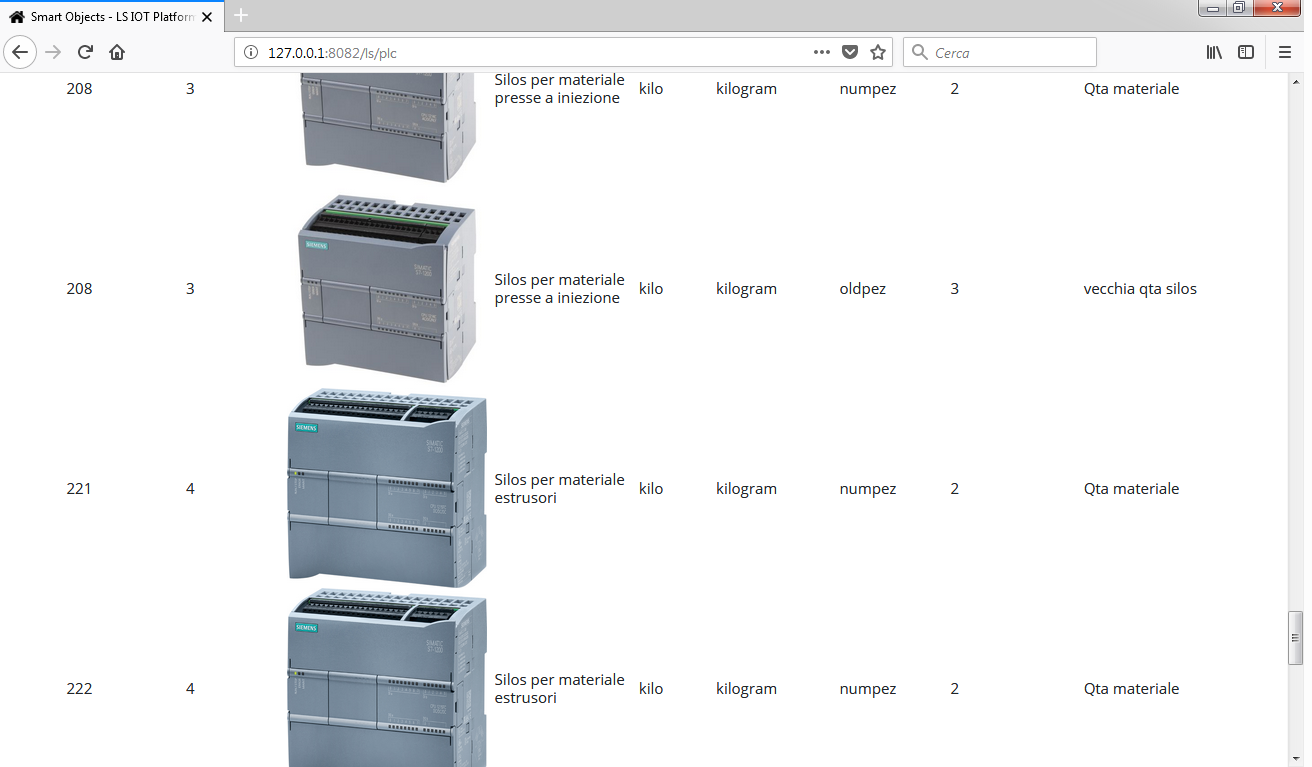
\includegraphics[width=1\textwidth]{images/SmartObjectsPlatform.png}
\end{frame}

\begin{frame}
\frametitle{Subscribe Rule}
\begin{itemize}
	\item messaggio json da inviare per usare il servizio push
	\item l'utente specifica la condizione
	\begin{itemize}
		\item nome e IP applicazione
		\item coda o topic activemq
		\item subscribe rule
		\begin{itemize}
			\item nome tabella da interrogare
			\item lista dei campi da monitorarne i cambiamenti
			\item espressione CRON
			\item clausola where
			
		\end{itemize}
	\end{itemize}
\end{itemize}
\end{frame}

\begin{frame}
\frametitle{Clausola where}
\begin{itemize}
	\item condition
	\begin{itemize}
		\item insieme di oggetti avro annidati
	\end{itemize}
	\item formula
	\begin{itemize}
		\item semplice stringa (per NAV)
	\end{itemize}
\end{itemize}
\end{frame}

\begin{frame}
\frametitle{Albero della condition}
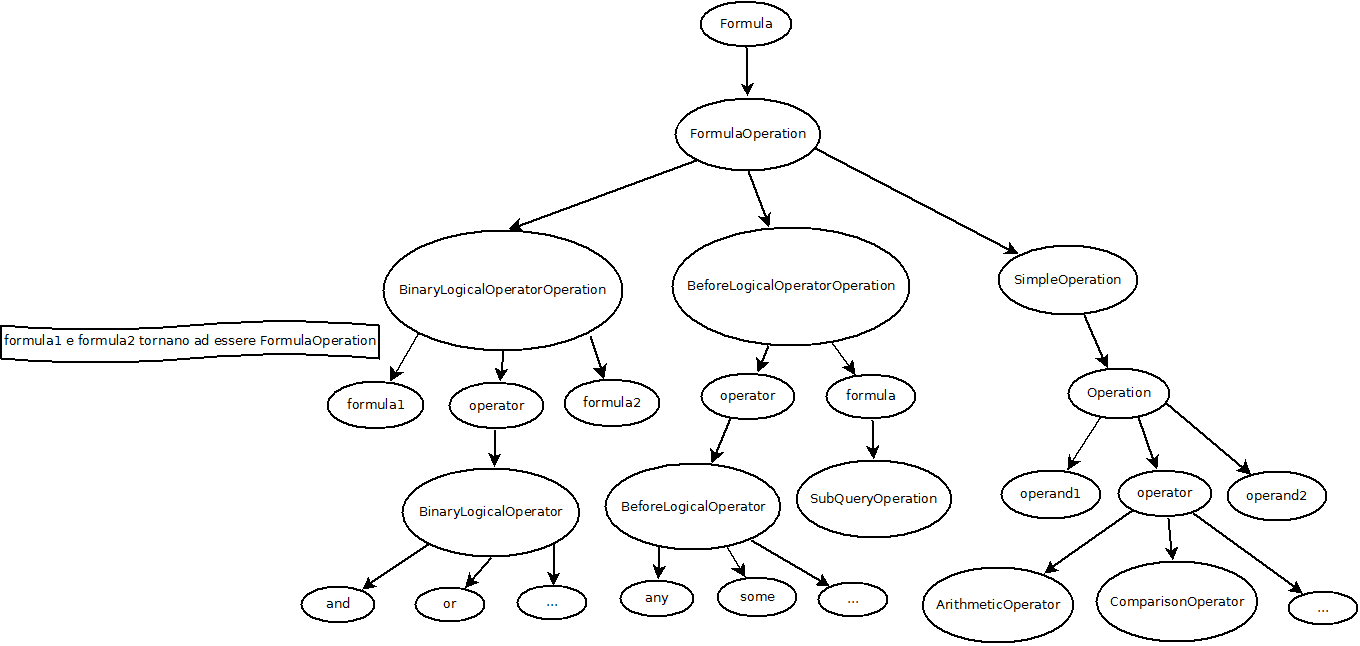
\includegraphics[width=1\textwidth]{images/struttura-query-tree.png}
\end{frame}

\begin{frame}
\frametitle{Subscriberule di una applicazione}
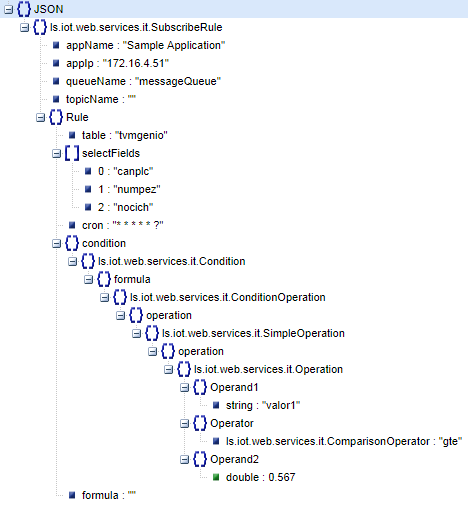
\includegraphics[width=0.6\textwidth]{images/subscribe-json-1.png}
\end{frame}

\begin{frame}
\frametitle{Regole nel database}
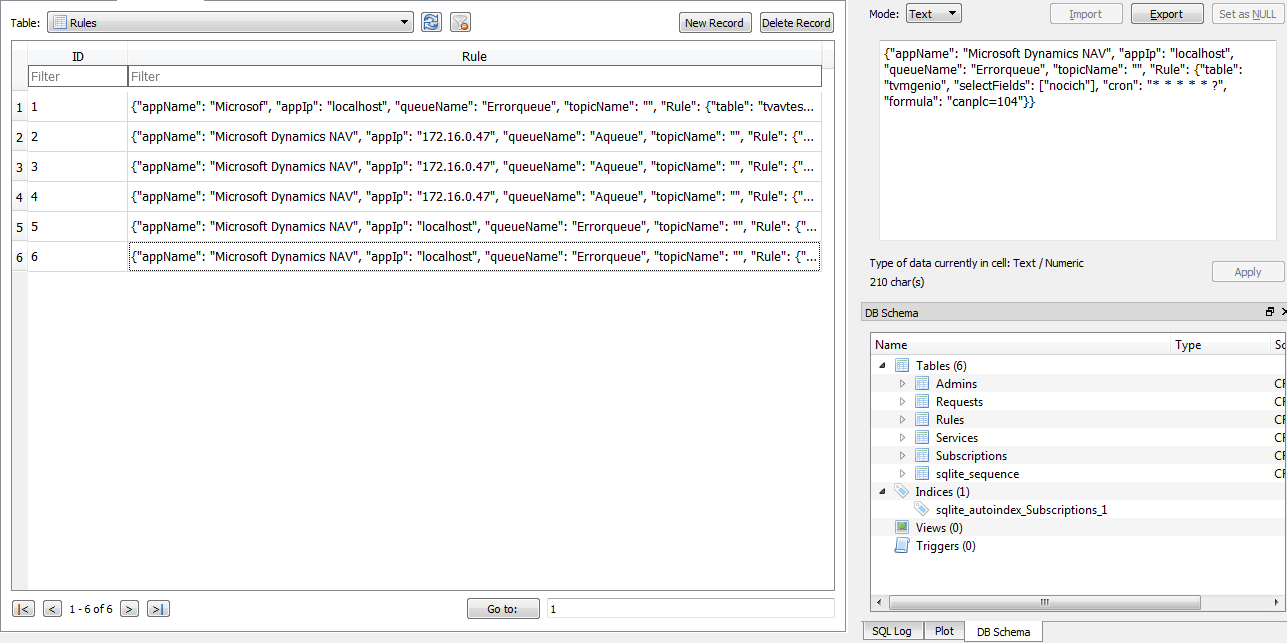
\includegraphics[width=1\textwidth]{images/DBPlatform1.png}
\end{frame}

\begin{frame}
\frametitle{Schema JSON Subscribe di NAV}
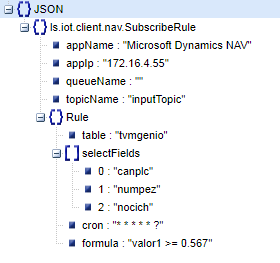
\includegraphics[width=0.6\textwidth]{images/subscribe-json-2.png}
\end{frame}

\begin{frame}
\frametitle{Class Diagram Subscribe Rule Interface}
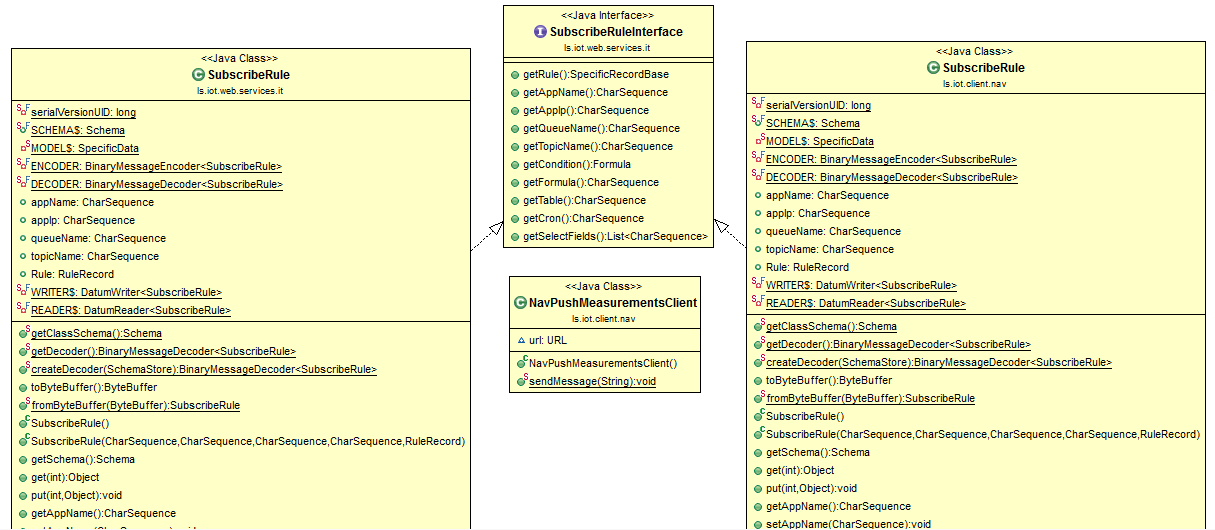
\includegraphics[width=1\textwidth]{images/ClassDiagram7.png}
\end{frame}

\begin{frame}
\frametitle{Class Diagram RetrievedDataInterface 1}
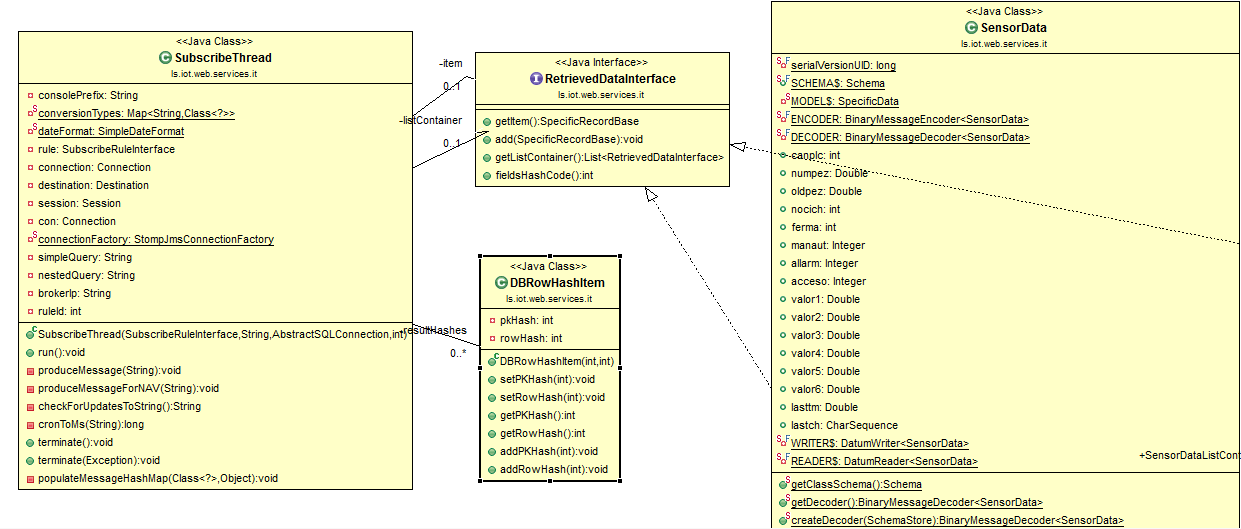
\includegraphics[width=1\textwidth]{images/ClassDiagram2.png}
\end{frame}

\begin{frame}
\frametitle{Class Diagram RetrievedDataInterface 2}
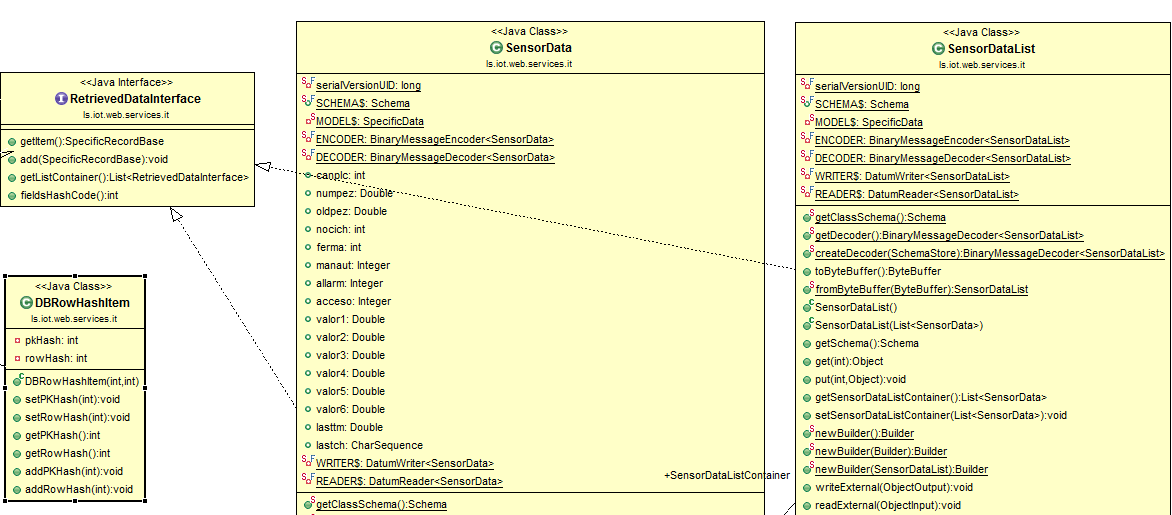
\includegraphics[width=1\textwidth]{images/ClassDiagram1.png}
\end{frame}

\begin{frame}
\frametitle{metodo di popolamento dati json}
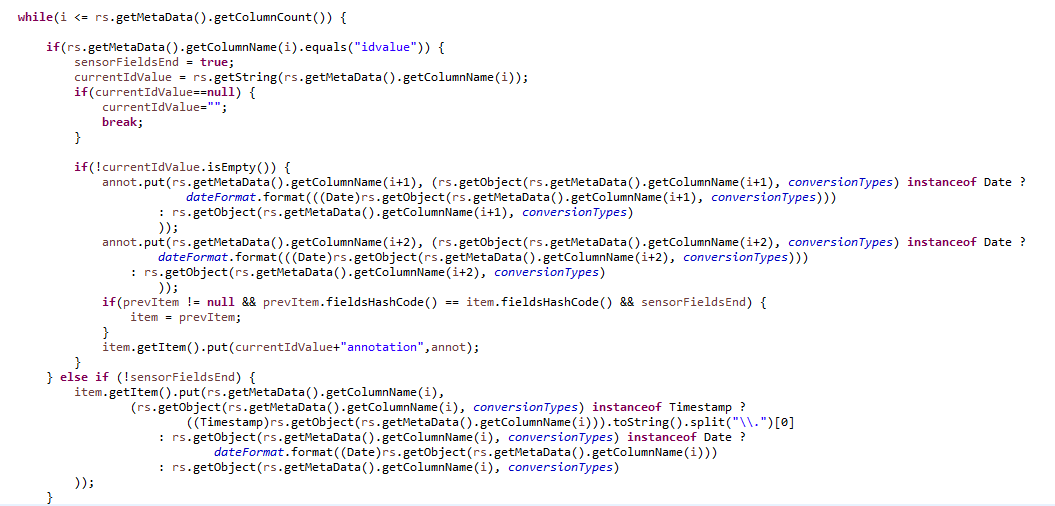
\includegraphics[width=1\textwidth]{images/popolamento-json.png}
\end{frame}

\begin{frame}
\frametitle{Class Diagram AbstractConnection}
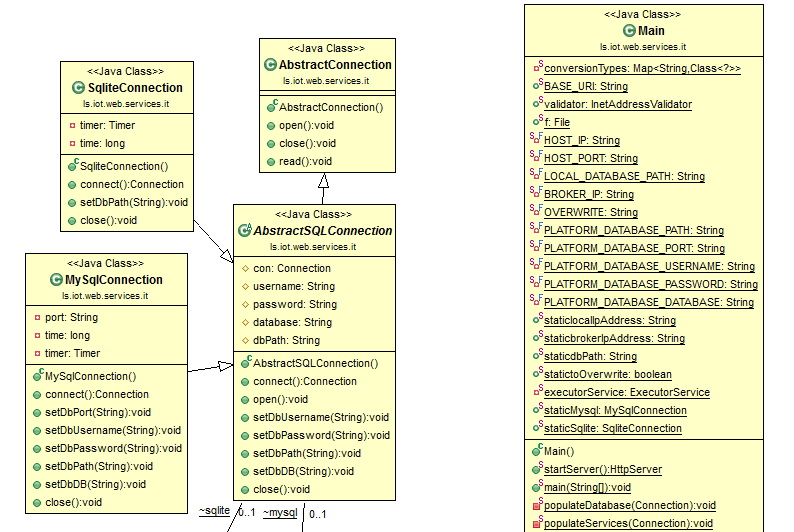
\includegraphics[width=1\textwidth]{images/main.png}
\end{frame}

%-------------------------inizio client-----------------------------

\begin{frame}
\frametitle{Client NAV}
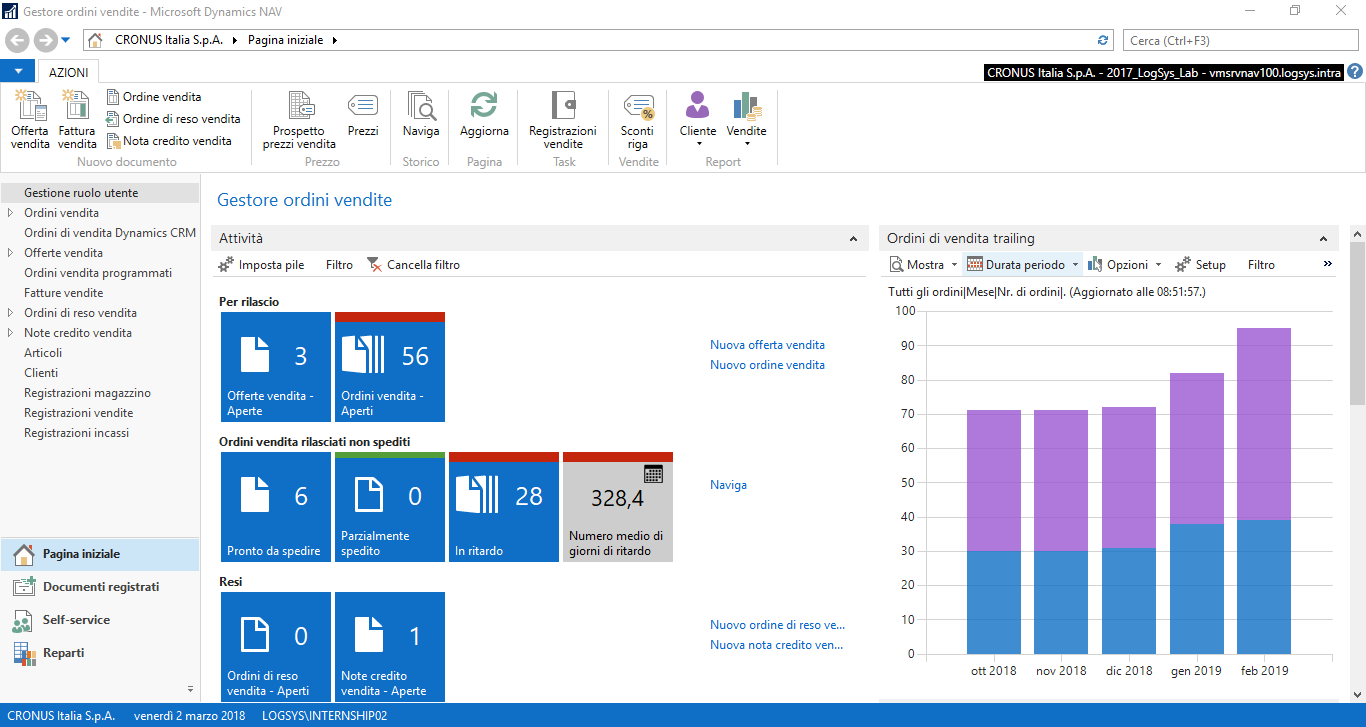
\includegraphics[width=1\textwidth]{images/NAVClient.png}
\end{frame}

\begin{frame}
\frametitle{Ambiente di sviluppo NAV}
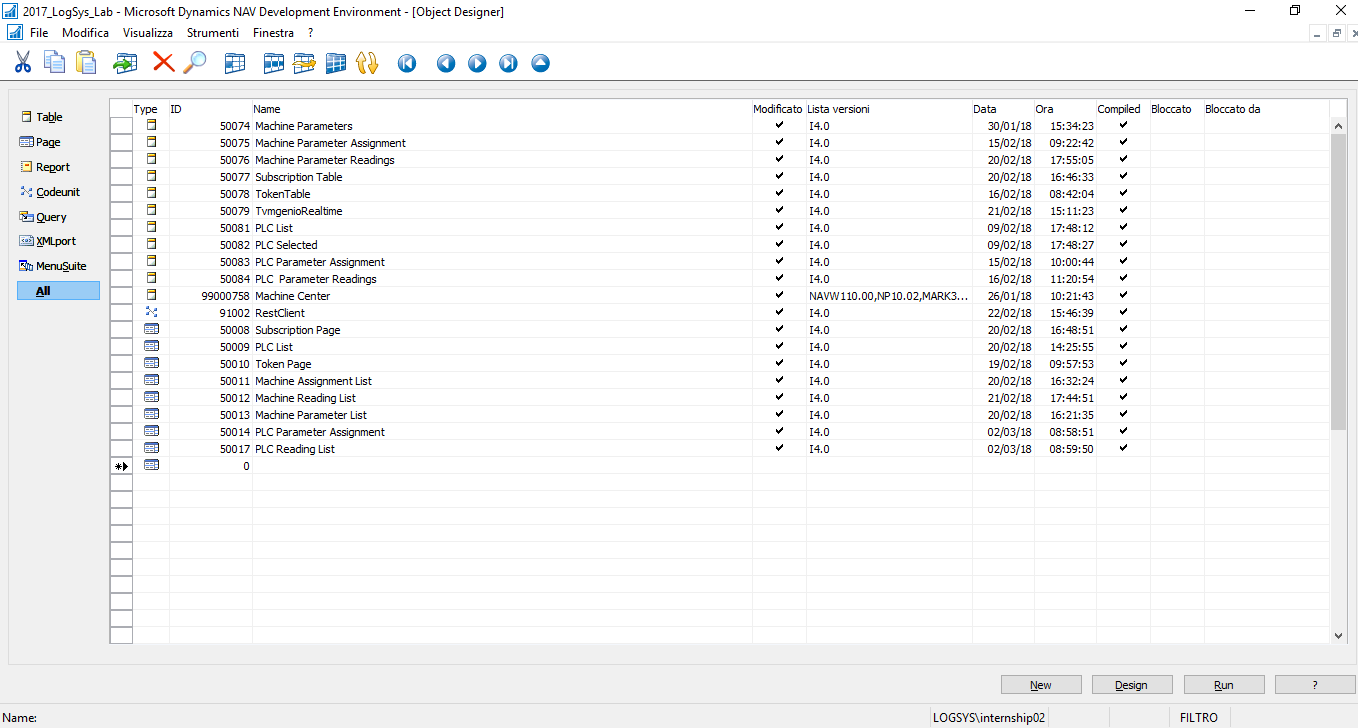
\includegraphics[width=1\textwidth]{images/NAVDevelopmentEnvironment.png}
\end{frame}


\begin{frame}
\frametitle{Class Diagram Client 1}
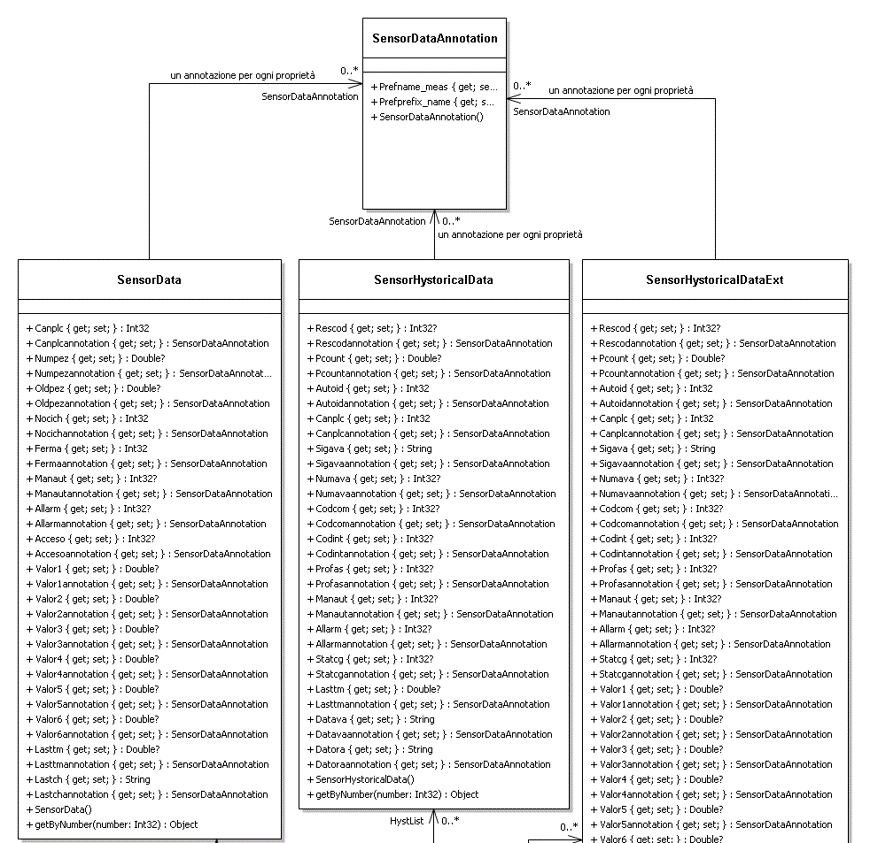
\includegraphics[width=0.6\textwidth]{images/ClassDiagramParte1.png}
\end{frame}

\begin{frame}
	\frametitle{Class Diagram Client 2}
	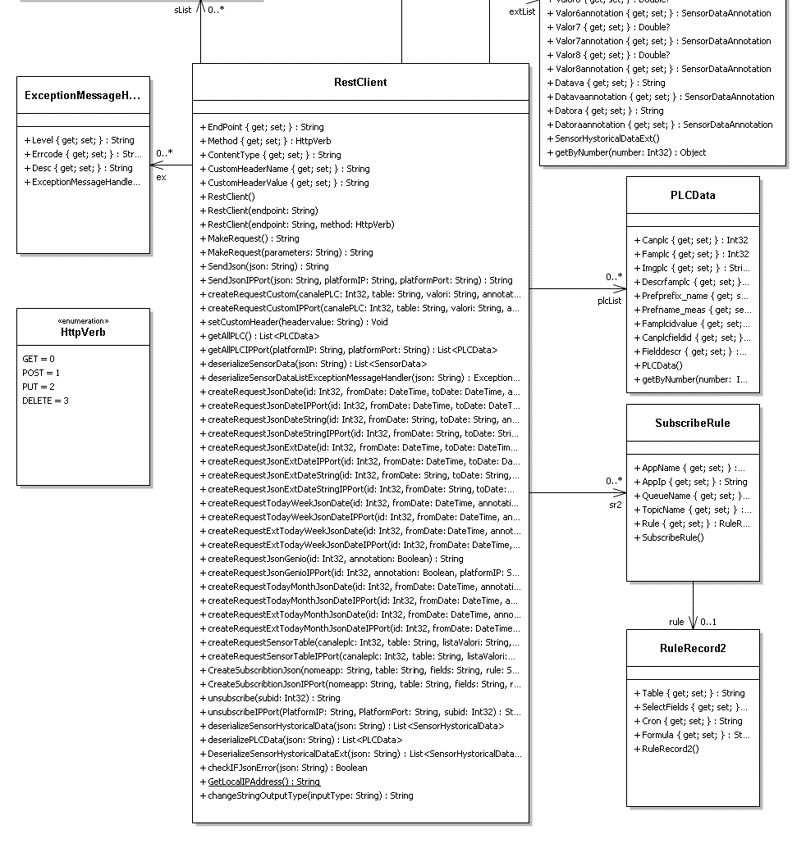
\includegraphics[width=0.6\textwidth]{images/ClassDiagramParte2.png}
\end{frame}

\begin{frame}
\frametitle{Lista con i parametri}
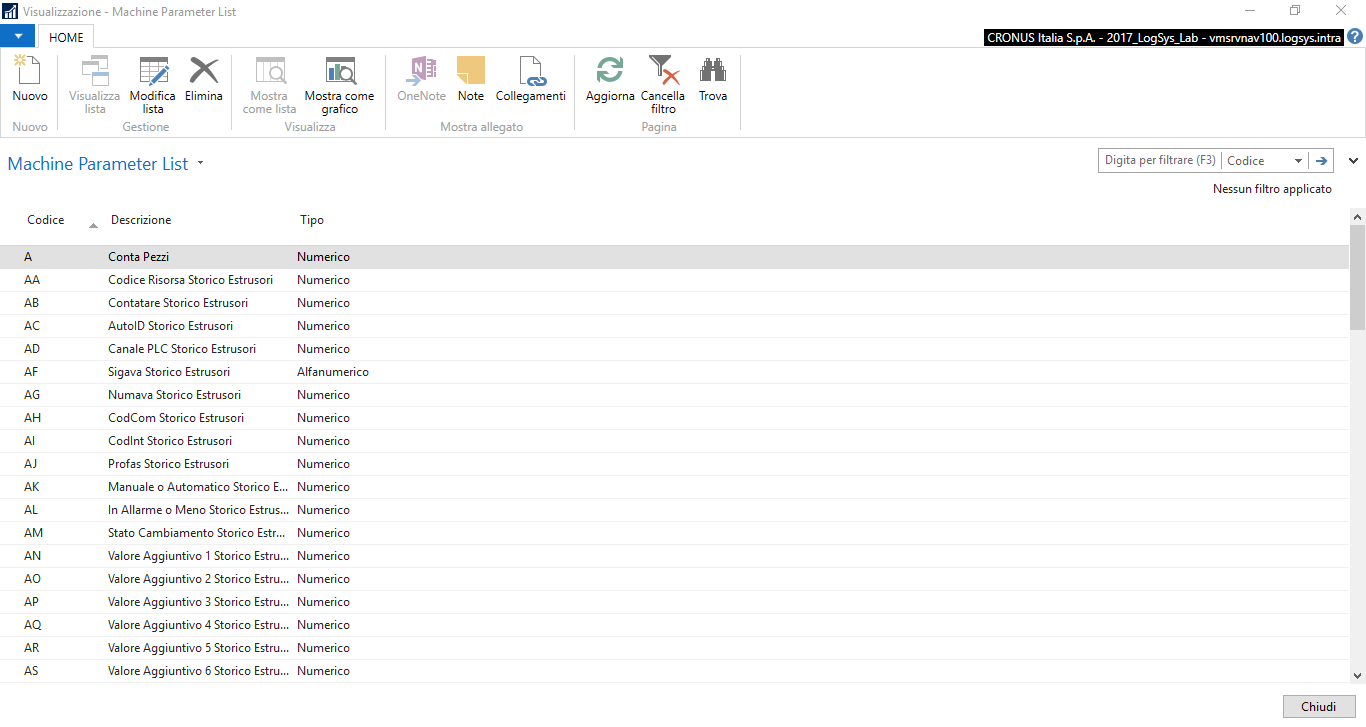
\includegraphics[width=1\textwidth]{images/MachineParameter.png}
\end{frame}

\begin{frame}
\frametitle{Metodo PushMeasurament 1}
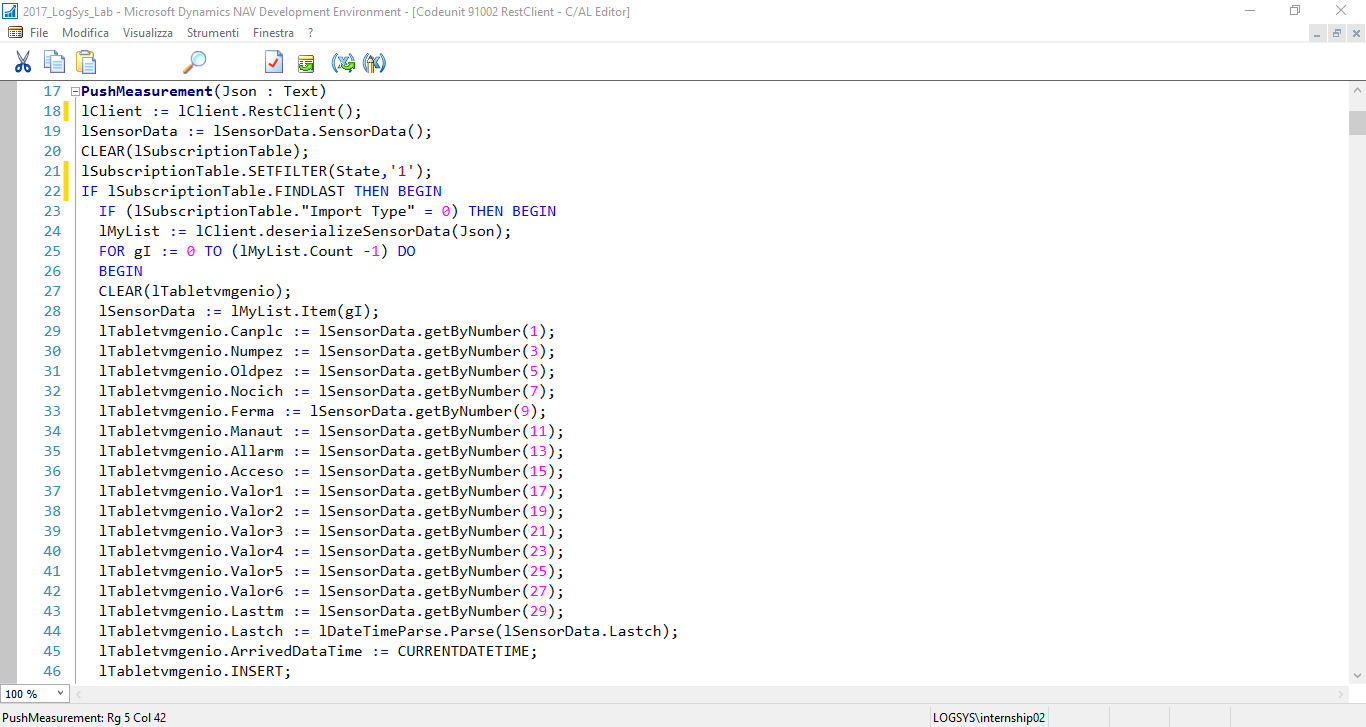
\includegraphics[width=1\textwidth]{images/NAVPushMeasuraments1.png}
\end{frame}

\begin{frame}
\frametitle{Metodo PushMeasurament 2}
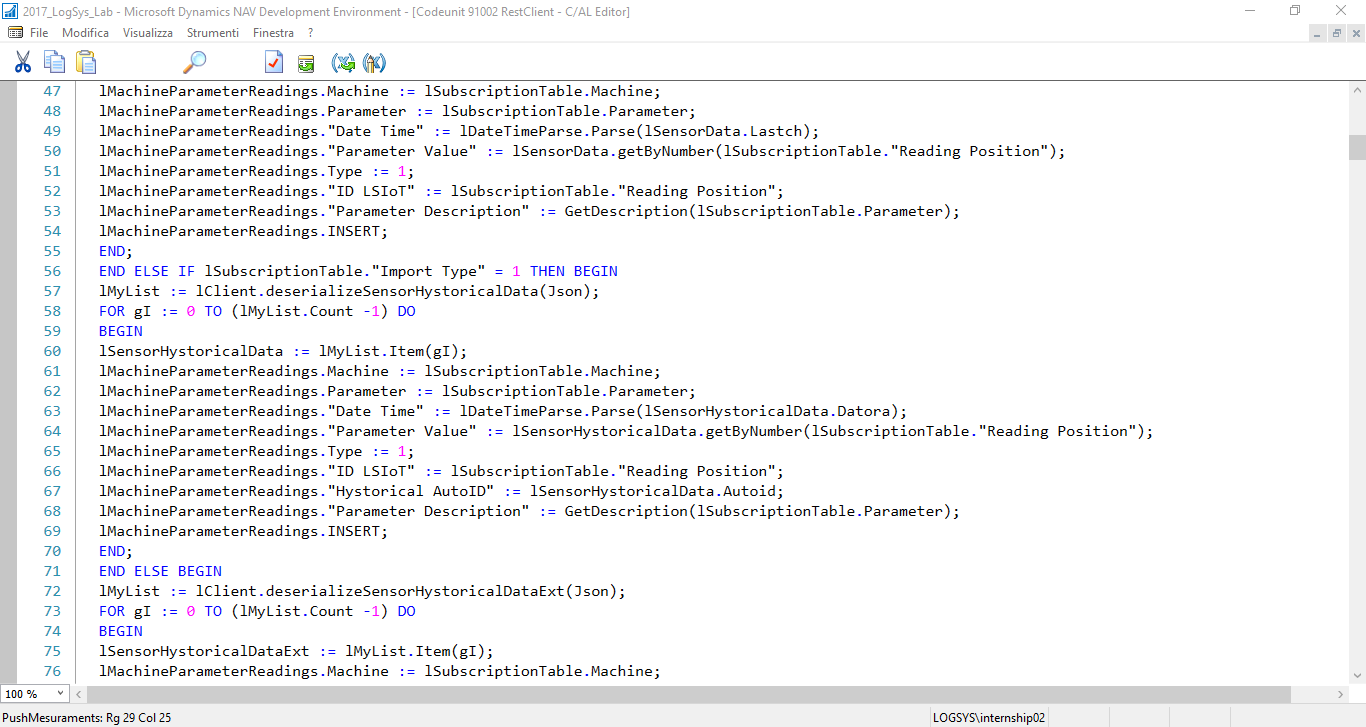
\includegraphics[width=1\textwidth]{images/NAVPushMeasuraments2.png}
\end{frame}

\begin{frame}
\frametitle{Metodo PushMeasurament 3}
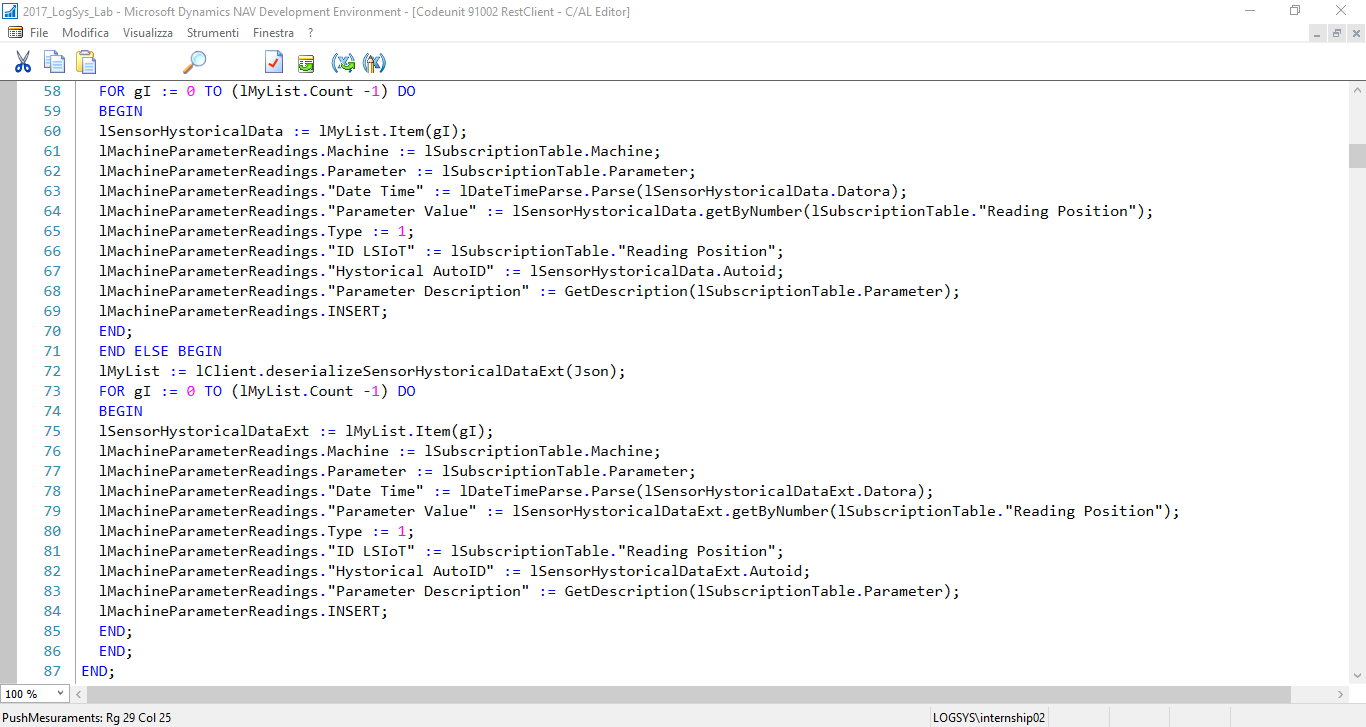
\includegraphics[width=1\textwidth]{images/NAVPushMeasuraments3.png}
\end{frame}

\begin{frame}
\frametitle{Lista delle funzioni della codeunit}
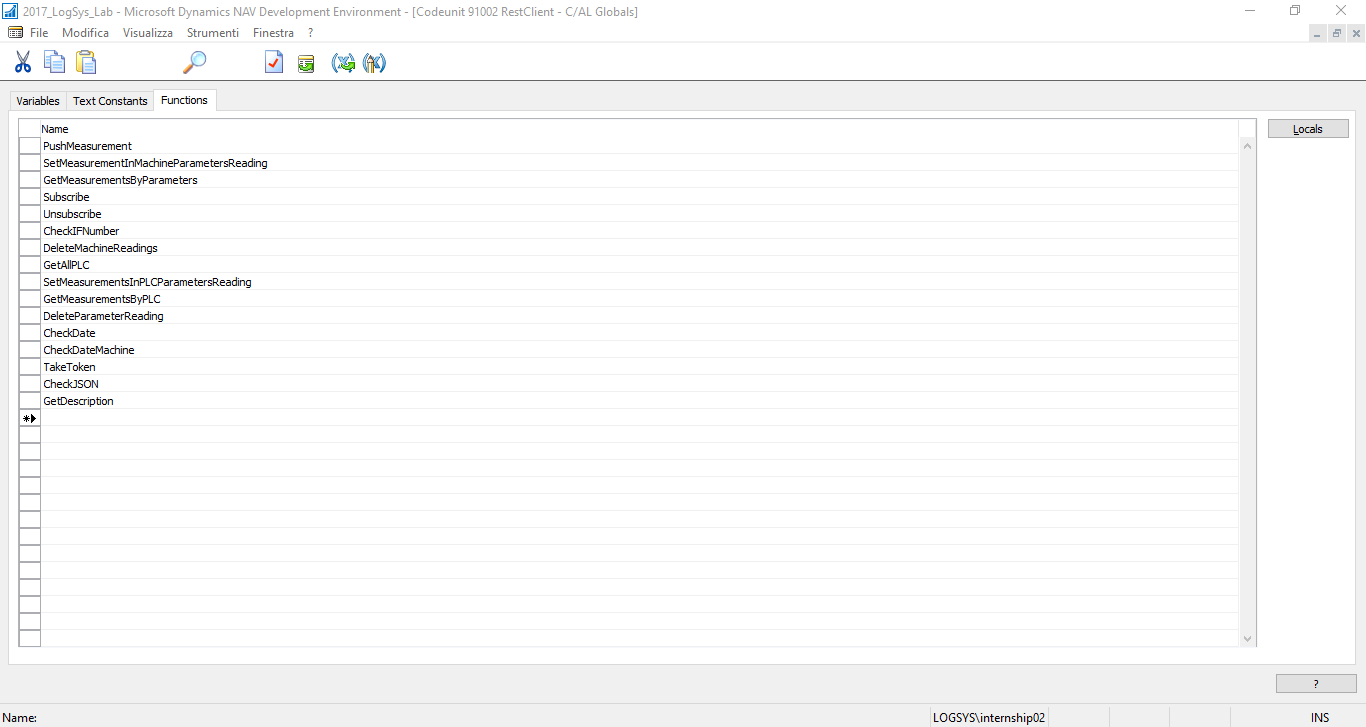
\includegraphics[width=1\textwidth]{images/NAVFunctionList.png}
\end{frame}


\begin{frame}
\frametitle{NAV servizi web}
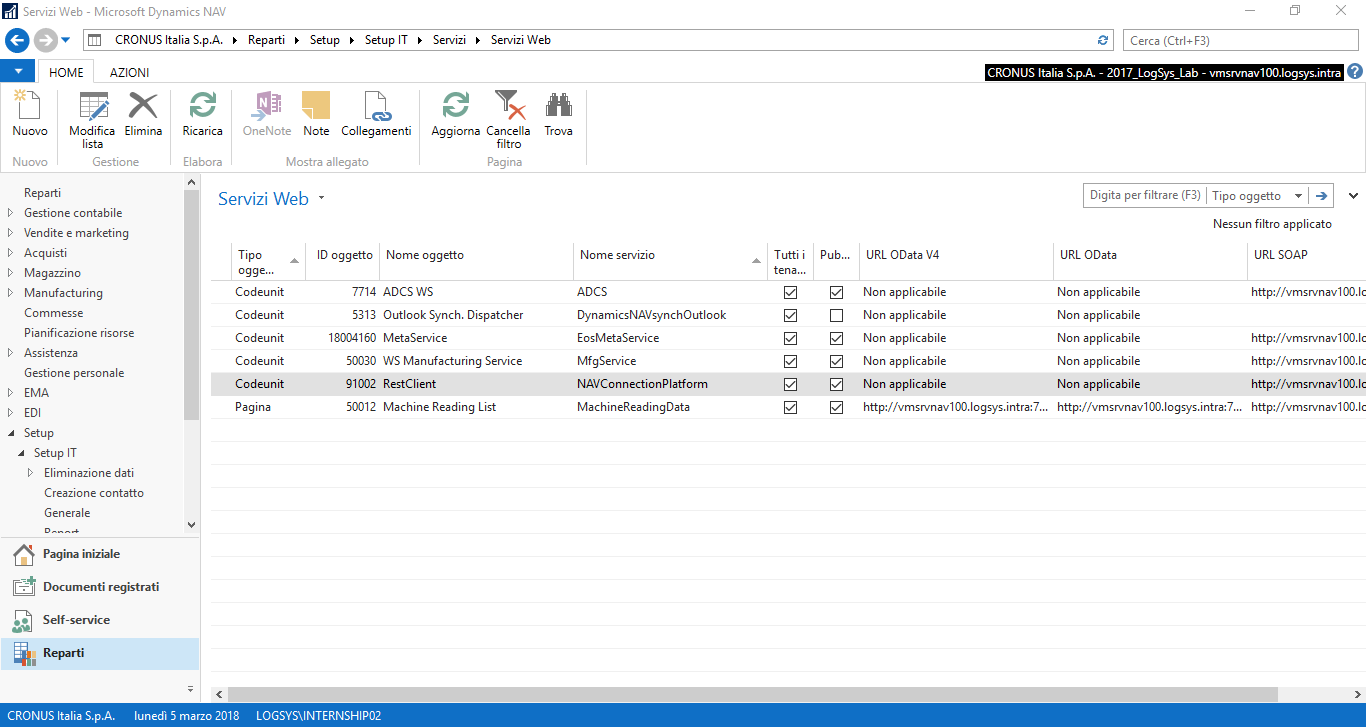
\includegraphics[width=1\textwidth]{images/NAVServiziWeb.png}
\end{frame}

\begin{frame}
\frametitle{Metodo SetMeasuramentPLC}
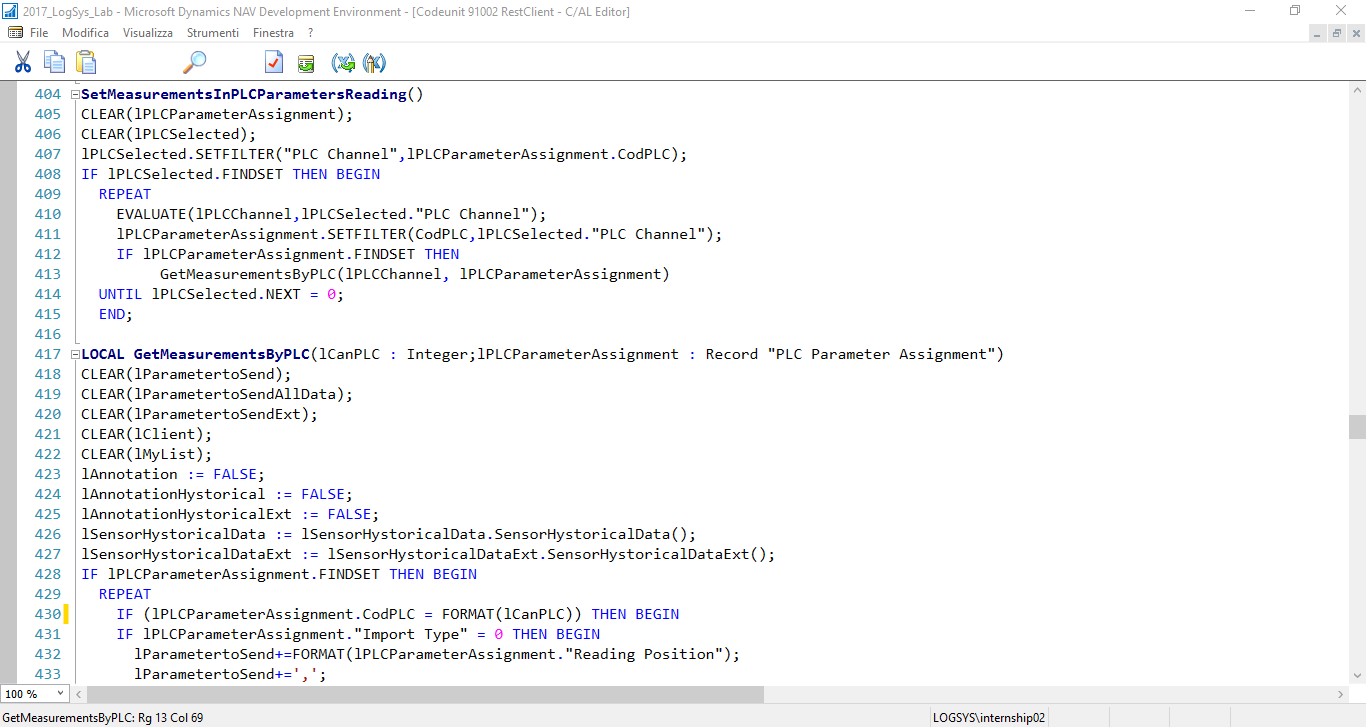
\includegraphics[width=1\textwidth]{images/NAVSetMesurament.png}
\end{frame}

\begin{frame}
\frametitle{NAV SubscriptionPage}
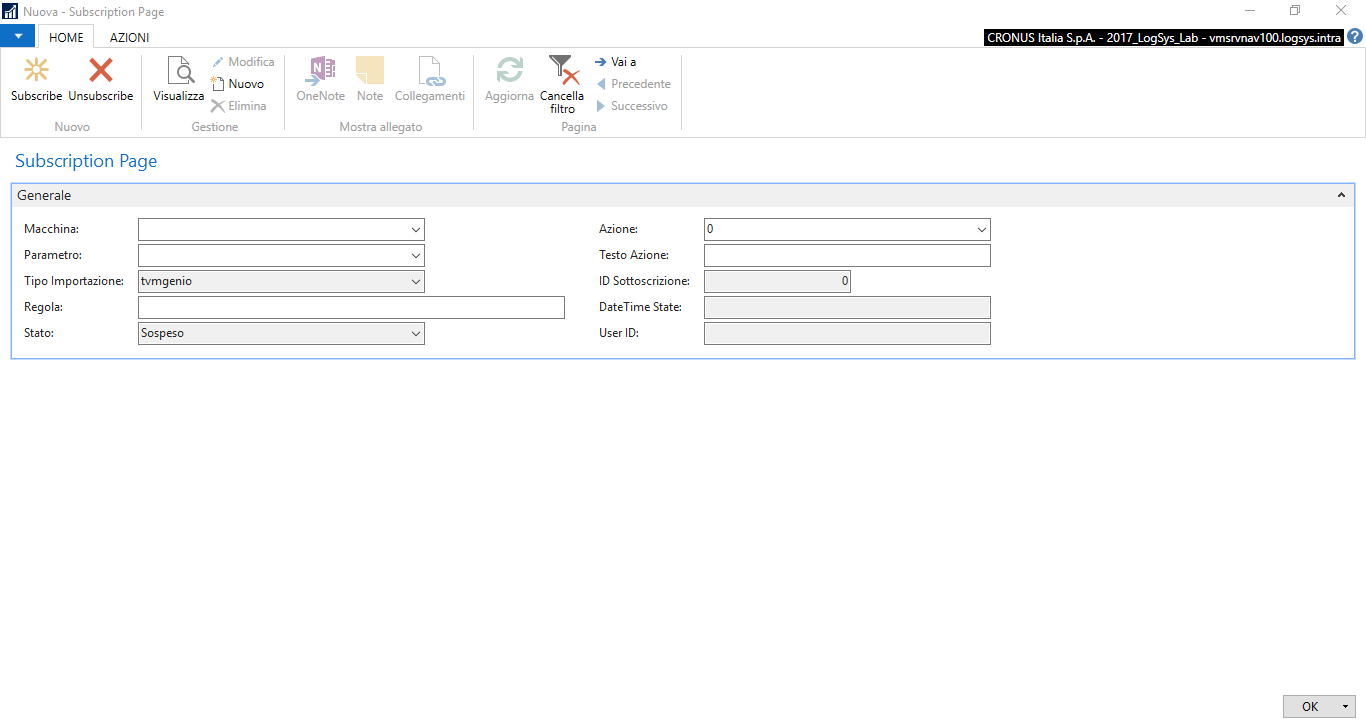
\includegraphics[width=1\textwidth]{images/NAVSubscriptionPage.png}
\end{frame}

\begin{frame}
\frametitle{PLC Assignment List}
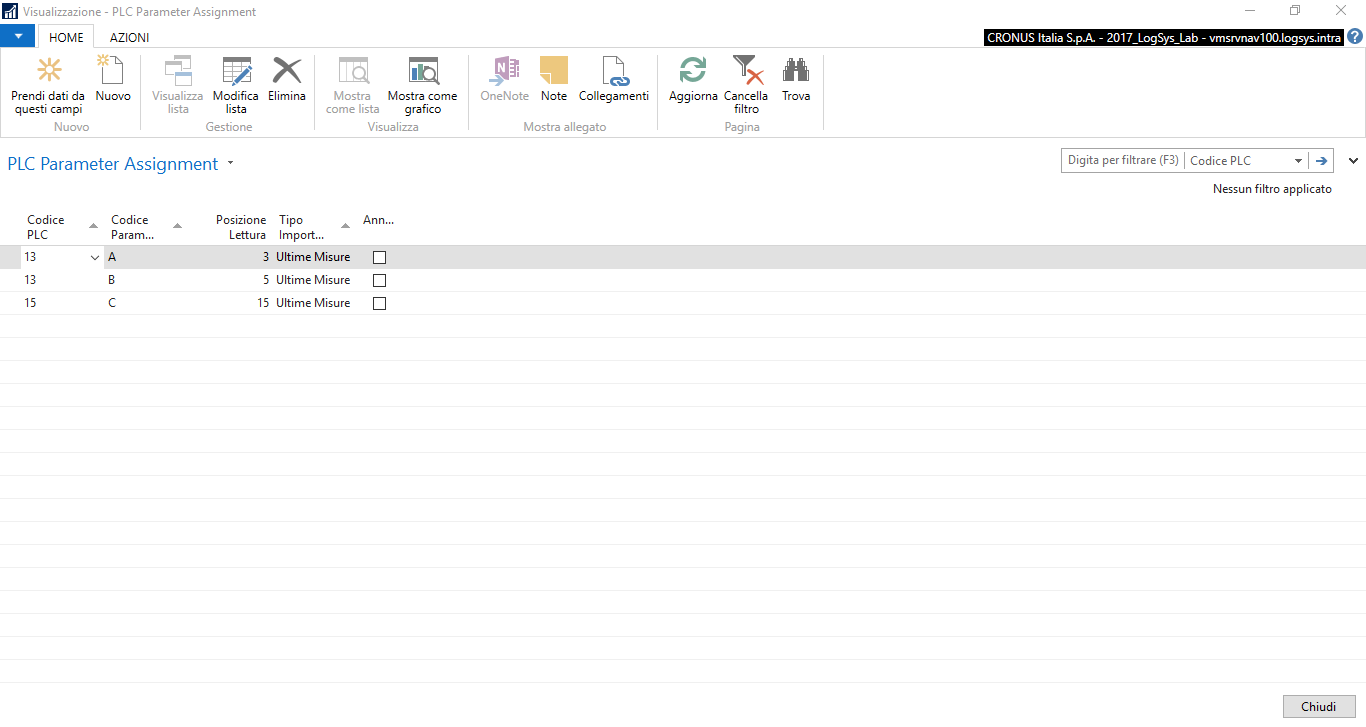
\includegraphics[width=1\textwidth]{images/PLCAssignmentList.png}
\end{frame}

\begin{frame}
\frametitle{Lista PLC}
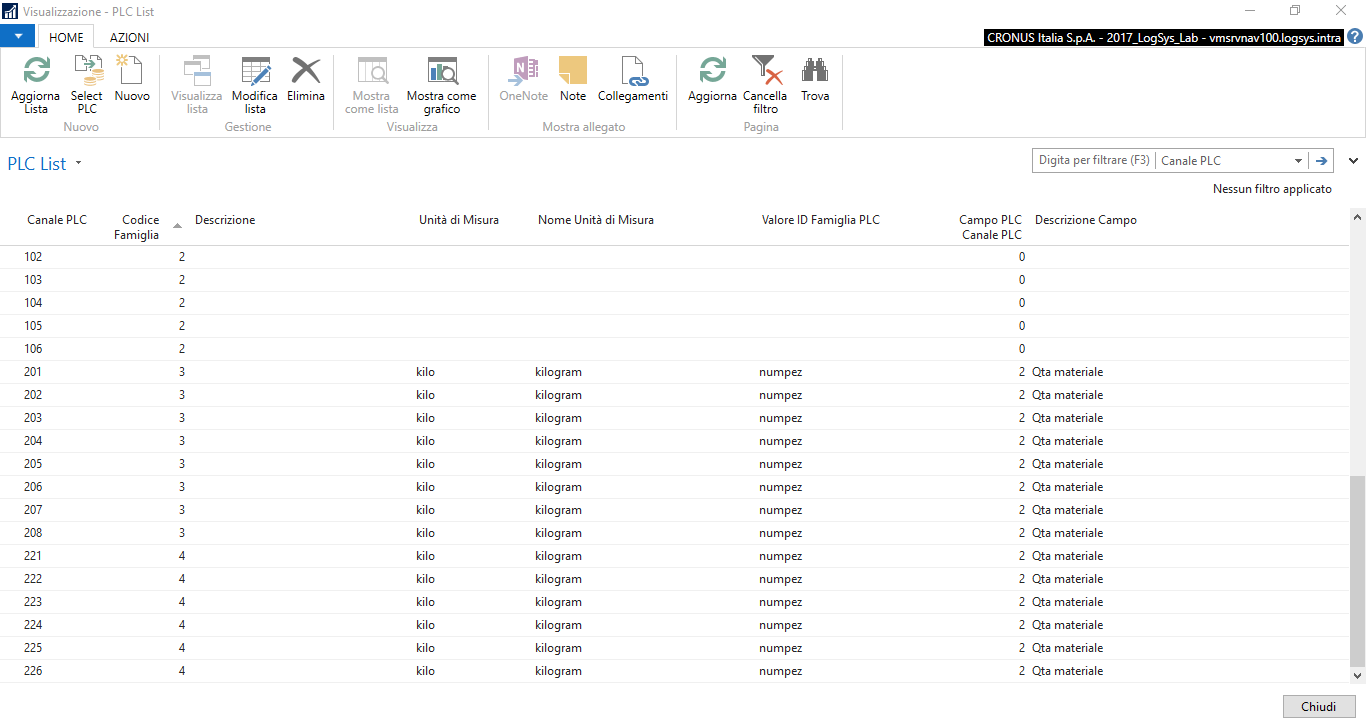
\includegraphics[width=1\textwidth]{images/PLCList.png}
\end{frame}

\begin{frame}
\frametitle{PLC Reading List}
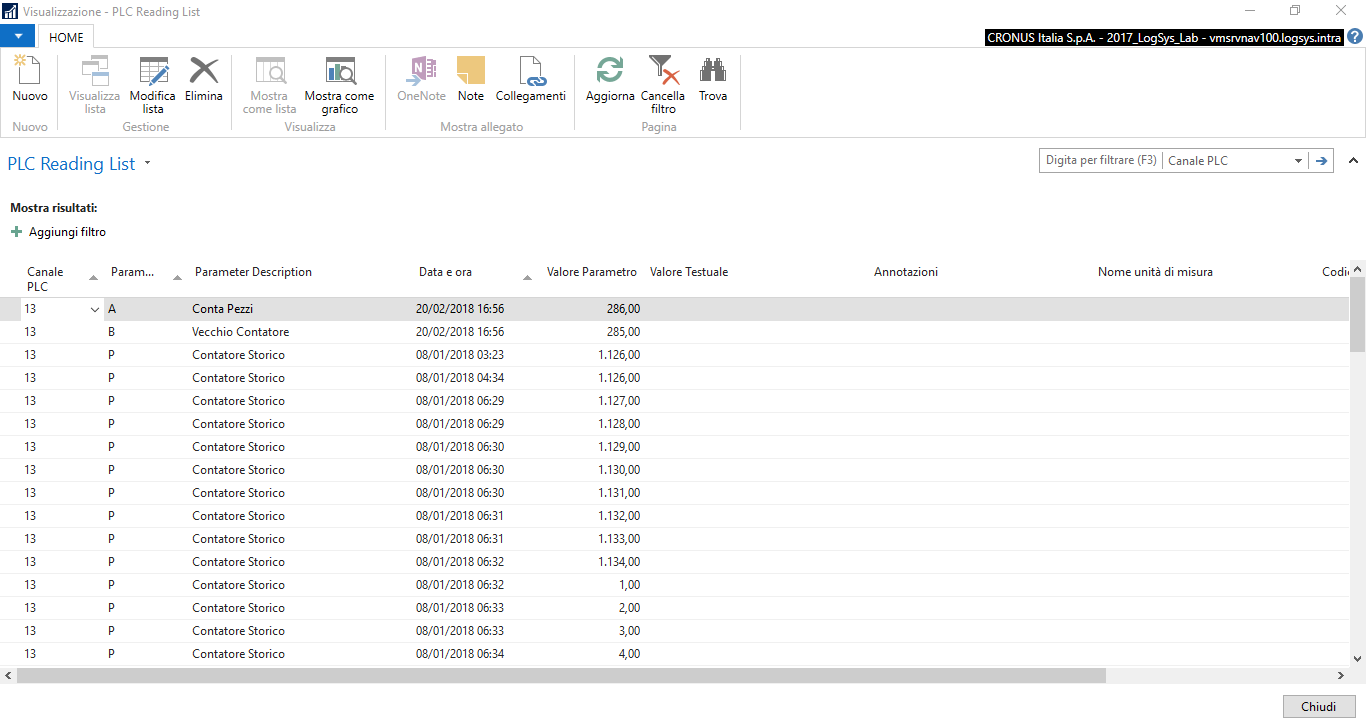
\includegraphics[width=1\textwidth]{images/PLCReadingList.png}
\end{frame}


\subsection{sub b}







\end{document}